\documentclass{article}
\usepackage[margin=7.5mm,paperwidth=10.5cm,paperheight=21.0cm]{geometry}
\usepackage[T1]{fontenc}
\usepackage[utf8]{inputenc}
\usepackage{graphicx}
\usepackage{graphbox}
\usepackage{xcolor}
\usepackage{listings}
\usepackage{multicol}
\usepackage{pgfornament}
\usepackage{ebgaramond}
\usepackage{pgfpages}
\usepackage{tikz}
\usepackage{tikzpagenodes}
\usepackage{comment}
\usetikzlibrary{chains}
\usepackage[a4,cam,cross]{crop}
\pgfpagesdeclarelayout{christmas}{
    \edef\pgfpageoptionheight{\the\paperheight}
    \edef\pgfpageoptionwidth{\the\paperwidth}
    \edef\pgfpageoptionborder{0pt}
}{  \pgfpagesphysicalpageoptions{
        logical pages=2,
        physical height=29.7cm,
        physical width=21.0cm
    }\pgfpageslogicalpageoptions{2}{
        border shrink=\pgfpageoptionborder,
        resized width=10.5cm, resized height=21.0cm,
        center=\pgfpoint{.25\pgfphysicalwidth}{.5\pgfphysicalheight}
    }\pgfpageslogicalpageoptions{1}{
        border shrink=\pgfpageoptionborder,
        resized width=10.5cm, resized height=21.0cm,
        center=\pgfpoint{.75\pgfphysicalwidth}{.5\pgfphysicalheight}
    }
}\pgfpagesuselayout{christmas}
\pagenumbering{gobble}
\definecolor{christmas}{HTML}{b12424}
\renewcommand{\c}[1]{{\color{christmas}#1}}
\lstset{
    language=TeX,
    morekeywords={begin,renewcommand,usepackage},
    basicstyle=\tiny\ttfamily,
    keywordstyle=\color{christmas},
    commentstyle=\color{darkgray}
}

% Source code also found on: https://github.com/Kamik423/christmas-card-2019
\begin{document}

\begin{tikzpicture}[remember picture, overlay, start chain, node distance=-2mm]

    \node (nworn) [shift={(9.5 mm,-9.5mm)}, anchor=north west, on chain ] at (-2.1,2){\pgfornament[width= 9.5 mm]{61}};
    \foreach \i in {1,...,4}
      {\node [on chain] {\pgfornament[width= 9.5mm]{62}};
      \node [on chain] {\pgfornament[width= 9.5mm]{61}};}
    \node (neorn) [on chain] {\pgfornament[width= 9.5 mm]{62}};
    \foreach \i in {1,...,9}
      {\node [continue chain=going below, on chain] {\pgfornament[width=9.5mm,symmetry=h]{62}};
      \node [continue chain=going below, on chain] {\pgfornament[width=9.5mm]{62}};}
    \node (seorn) [on chain] {\pgfornament[width=9.5mm,symmetry=h]{62}};
    \foreach \i in {1,...,4}
      {\node [continue chain=going left, on chain] {\pgfornament[width=9.5mm,symmetry=h]{61}};
      \node [continue chain=going left, on chain] {\pgfornament[width= 9.5mm,symmetry=h]{62}};}
    \node (sworn) [on chain] {\pgfornament[width= 9.5mm,symmetry=h]{61}};
    \foreach \i in {1,...,9}
      {\node [continue chain=going above, on chain] {\pgfornament[width=9.5mm]{61}};
      \node [continue chain=going above, on chain] {\pgfornament[width=9.5mm,symmetry=h]{61}};}
\end{tikzpicture}

\begin{comment}
\begin{tikzpicture}[remember picture, overlay]
    \node[anchor=north west] at (current page text area.north west) {%
        \pgfornament[width=1.5cm]{61}};
    \node[anchor=north east] at (current page text area.north east) {%
        \pgfornament[width=1.5cm, symmetry=v]{61}};
    \node[anchor=south west] at (current page text area.south west) {%
        \pgfornament[width=1.5cm,symmetry=h]{61}};
    \node[anchor=south east] at (current page text area.south east) {%
        \pgfornament[width=1.5cm,symmetry=c]{61}};
\end{tikzpicture}
\end{comment}
\centering

\vspace{1 cm}

{\huge \c{H}appy \c{V}alentine's \c{D}ay!\\[5mm]}

{\parindent=0pt
 \newcommand{\shiftleft}{\hspace*{-0.5\dimexpr\csname Gm@layoutwidth\endcsname-\textwidth\relax}}

\shiftleft
\includegraphics[width=5cm]{aj}\shiftleft\vfill

\shiftleft
\includegraphics[width=5cm]{heart}\shiftleft\vfill

\shiftleft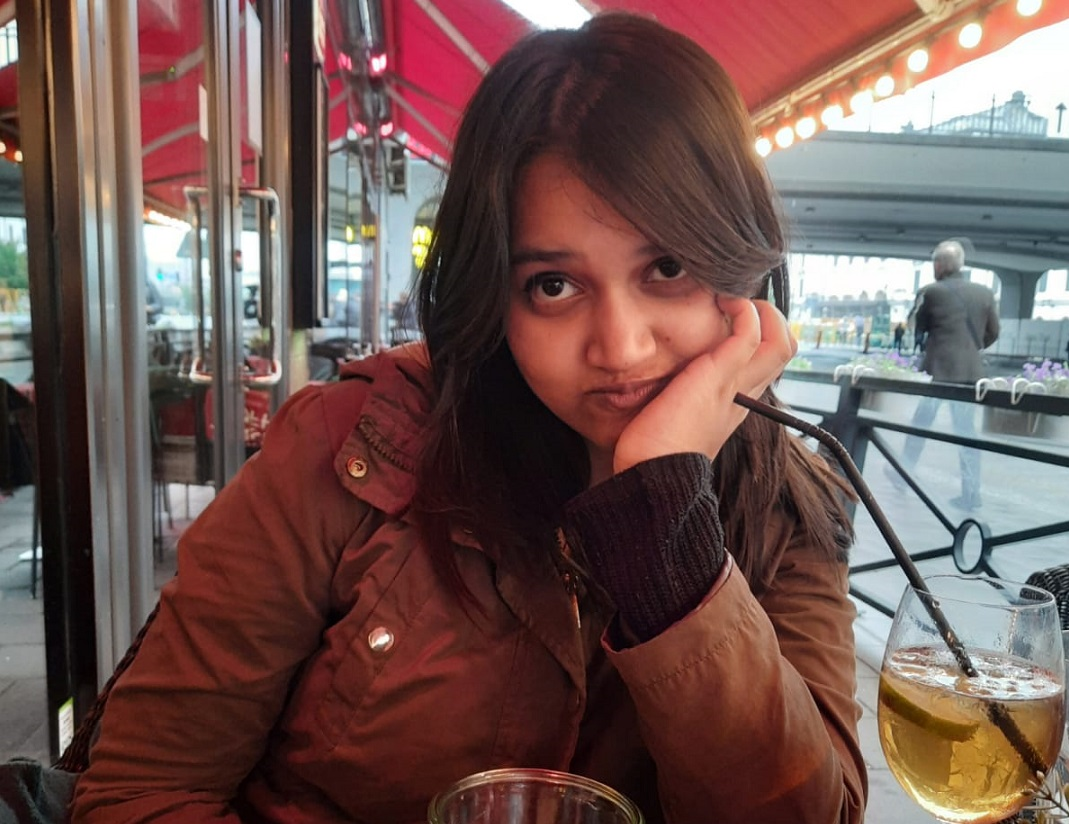
\includegraphics[width=5cm]{ng_cute}\shiftleft

}

\begin{comment}
  \centering
  
\includegraphics[align=c,height= 5 cm, width = 5 cm]{aj} 
  \hspace*{.2in}
 
\begin{tikzpicture}
\centering
  \draw[red,fill=red] (0,0) .. controls (0,0.75) and (-1.5,1.00) .. (-1.5,2)  arc (180:0:0.75)  -- cycle;
  \draw[red,fill=red] (0,0) .. controls (0,0.75) and ( 1.5,1.00) .. ( 1.5,2)  arc (0:180:0.75) -- cycle;
\end{tikzpicture}

  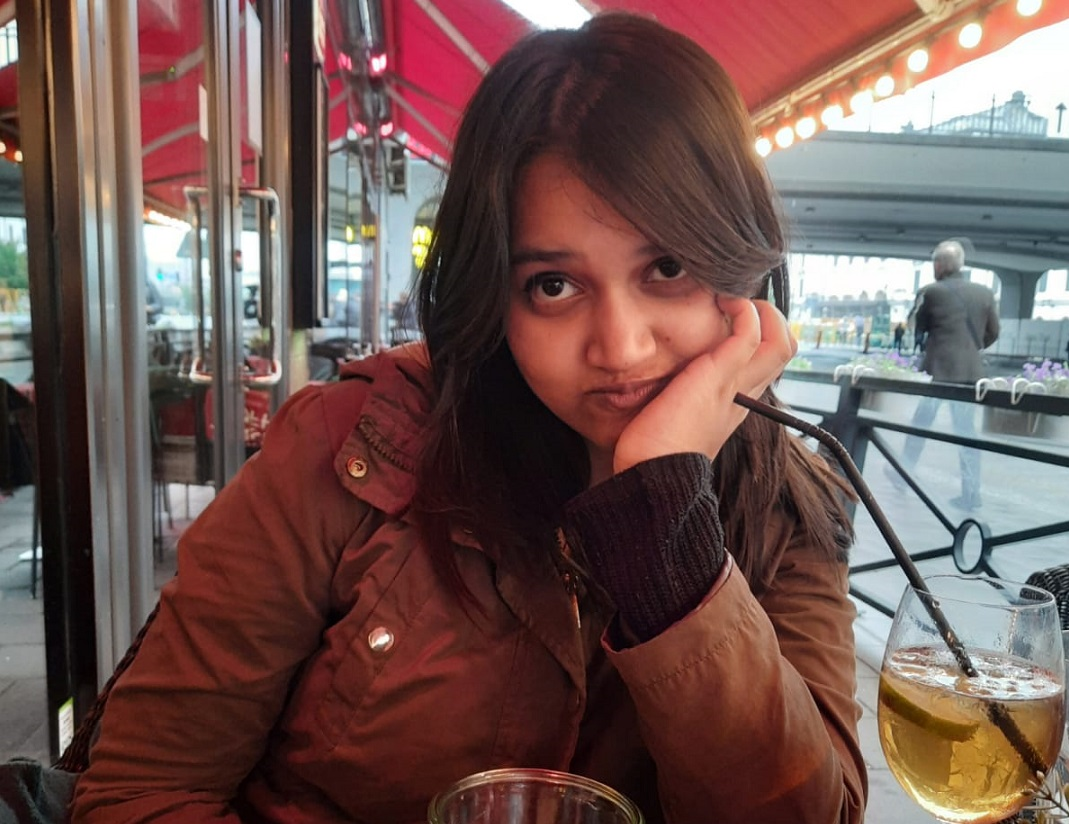
\includegraphics[align=c,height= 5 cm, width = 5 cm]{ng_cute}
\end{comment}

%\hspace{1cm}
\includegraphics[width = 4 cm, height = 4 cm]{aj}
% Cat sourced from:
% https://www.reddit.com/r/MedievalCats/comments/e713ht/king_derpy/
% Edited version on:
% https://github.com/Kamik423/christmas-card-2019
\vfill
%\hspace{1cm}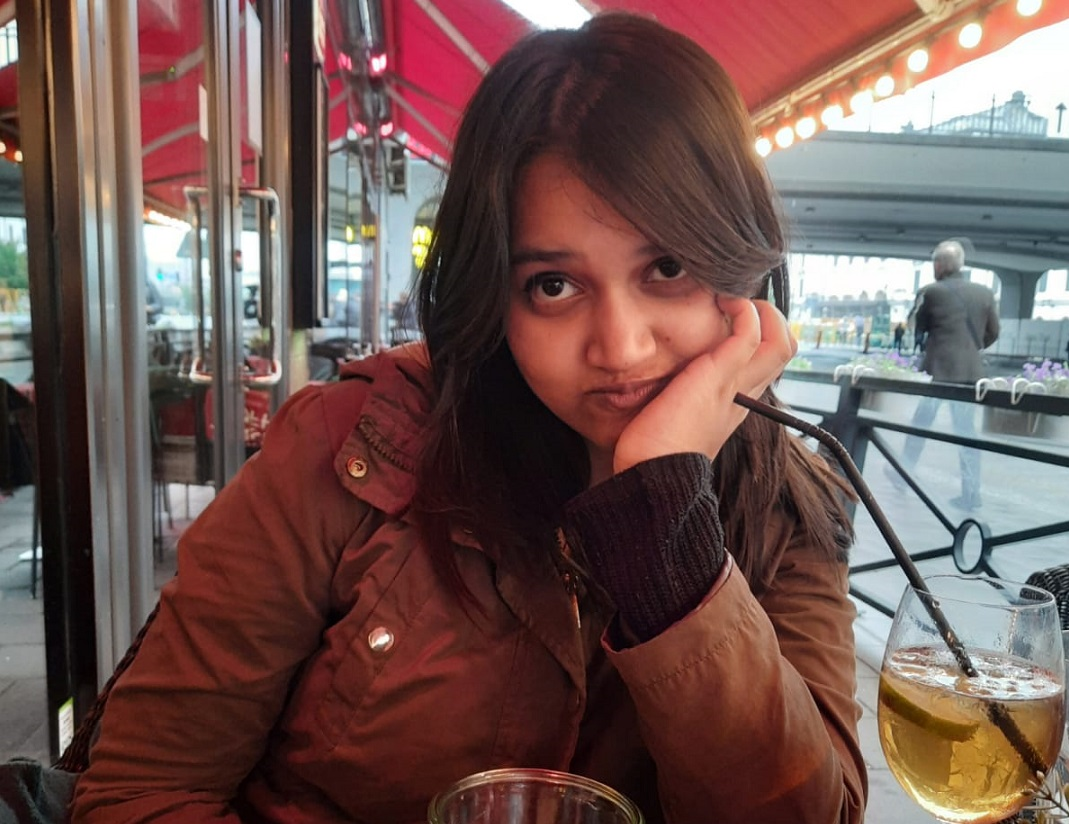
\includegraphics[width = 4 cm, height = 4 cm]{ng_cute}

\begin{comment}
\vfill
\begin{minipage}[c]{.8\textwidth}
    \centering
    \large
    \c{``}Give a man a fire and he's warm for a day, but set fire to him
    and he's warm for the rest of his life.\c{''}\\[5mm]
    \c{--}Sir Terry Pratchett
\end{minipage}
\end{comment}
\vfill
\newpage %%%%%%%%%%%%%%%%%%%%%%%%%%%%%%%%%%%%%%%%%%%%%
%\lstinputlisting{christmas-card-2019.tex}

\begin{tikzpicture}[remember picture, overlay, start chain, node distance=-2mm]

    \node (nworn) [shift={(9.5 mm,-9.5mm)}, anchor=north west, on chain ] at (-6,2){\pgfornament[width= 9.5 mm]{61}};
    \foreach \i in {1,...,4}
      {\node [on chain] {\pgfornament[width= 9.5mm]{62}};
      \node [on chain] {\pgfornament[width= 9.5mm]{61}};}
    \node (neorn) [on chain] {\pgfornament[width= 9.5 mm]{62}};
    \foreach \i in {1,...,9}
      {\node [continue chain=going below, on chain] {\pgfornament[width=9.5mm,symmetry=h]{62}};
      \node [continue chain=going below, on chain] {\pgfornament[width=9.5mm]{62}};}
    \node (seorn) [on chain] {\pgfornament[width=9.5mm,symmetry=h]{62}};
    \foreach \i in {1,...,4}
      {\node [continue chain=going left, on chain] {\pgfornament[width=9.5mm,symmetry=h]{61}};
      \node [continue chain=going left, on chain] {\pgfornament[width= 9.5mm,symmetry=h]{62}};}
    \node (sworn) [on chain] {\pgfornament[width= 9.5mm,symmetry=h]{61}};
    \foreach \i in {1,...,9}
      {\node [continue chain=going above, on chain] {\pgfornament[width=9.5mm]{61}};
      \node [continue chain=going above, on chain] {\pgfornament[width=9.5mm,symmetry=h]{61}};}
      
\end{tikzpicture}

\centering

\vspace{1 cm}

{\huge \c{S}ending \c{H}ugs, \c{K}isses, \\[5mm]}

{\huge and \c{P}yaar}\\[5mm]

\begin{figure}[h]
\centering 

\includegraphics[width = 5 cm]{ajng}
    \caption{Bollywood star and boyfriend}
\end{figure}
%\vfill Typeset by Hans in EBGaramond in \LaTeX.

\vspace{0.5 cm}
{\huge to the \c{W}orld's }

\vspace{0.5 cm}

{\huge \c{L}ittlest \c{M}unchkin}

\vspace{2 cm}

\begin{minipage}[c]{.8\textwidth}
    \centering
    \large
    \c{``}Wild horses couldn't drag me away.\c{''}\\[5mm]
    
\end{minipage}
\end{document}


{\Huge\c{\&}}\\[5mm]
{\Large lots of hugs and kisses}\\[5mm]
{\Large wünscht euch \c{H}ans.}\\